\documentclass{amsart}

\usepackage{amsmath,amsthm,amssymb,tikz,hyperref,cleveref,CJKutf8}
\hypersetup{hidelinks}

\crefname{theorem}{Theorem}{Theorems}
\crefname{corollary}{Corollary}{Corollaries}
\crefname{figure}{Figure}{Figures}
\crefname{equation}{Equation}{Equations}
\crefname{remark}{Remark}{Remarks}
\crefname{section}{Section}{Sections}

\definecolor{oi-orange}{HTML}{E69F00}
\definecolor{oi-sky}{HTML}{56B4E9}
\definecolor{oi-green}{HTML}{009E73}
\definecolor{oi-yellow}{HTML}{F0E442}
\definecolor{oi-blue}{HTML}{0072B2}
\definecolor{oi-vermillion}{HTML}{D55E00}
\definecolor{oi-purple}{HTML}{CC79A7}

\newtheorem{theorem}{Theorem}
\newtheorem{corollary}[theorem]{Corollary}
\newtheorem{remark}{Remark}

\newcommand{\R}{\mathbb{R}}

\title{Degree-respecting labellings with ordered neighbour sums}
\author{T.~Uda}
\date{}

\subjclass[2020]{05C78, 05C07}
\keywords{graph labelling, vertex degrees, neighbour sums, finite minimisation}

\begin{document}
\begin{CJK*}{UTF8}{min}

\begin{abstract}
The motivating question comes from the enumeration of hydrocarbon graphs, where
vertices represent carbon atoms, hydrogen atoms are omitted, and edges represent
single carbon--carbon bonds. For every finite simple graph, every strictly
increasing real assignment of weights to its ordered labels admits a labelling
that orders vertices by non-increasing degree and, among vertices of equal degree,
gives the vertex with the larger label the smaller or equal weighted sum over its
neighbours. Theorem~\ref{thm:strict-weights} proves this statement for arbitrary
strictly increasing real weights, and Corollary~\ref{cor:powers-of-two} gives the
powers-of-two case. The proof chooses, among labellings that order vertices by
non-increasing degree, one minimizing the sum over edges of the products of the
endpoint weights.
\end{abstract}

\maketitle

\section{Introduction}

The motivating setting is the enumeration of hydrocarbon graphs, where vertices
represent carbon atoms, hydrogen atoms are omitted, and edges represent single
carbon--carbon bonds. For a graph with vertex set \(V\) and \(n=|V|\) vertices,
the convention with labels \(1,\ldots,n\) uses a bijection
\(V\to\{1,\ldots,n\}\); here we use the ordered label set
\[
  I_n=\{0,1,\ldots,n-1\}.
\]
For the labels in \(I_n\), assign weight \(2^i\) to label \(i\). The weighted
neighbour sum of a vertex is the sum of the weights assigned to its neighbours.
We seek a labelling that gives smaller labels to vertices of larger degree and,
among vertices of equal degree, gives the vertex with the larger label the
smaller or equal weighted neighbour sum.
Smooth Pudding describes this labelling question in a 2024 post
\cite{smooth-pudding-2024} and attributes it to an earlier post dated 29 May
2024.
The result applies to every finite simple graph, without connectedness or a
bound on the maximum degree, and allows the powers of two to be replaced by any
strictly increasing real weights. Theorem~\ref{thm:strict-weights} establishes
this statement, with the powers-of-two case as
Corollary~\ref{cor:powers-of-two}.

Morgan's canonical numbering of chemical structures also uses vertex labels
\cite{morgan-1965}. We instead study a labelling that orders vertices by degree
and, within each degree class, orders weighted neighbour sums.

\section{Preliminaries}

Let \(G=(V,E)\) be a finite simple undirected graph, and put \(n=|V|\). For
\(v\in V\), let \(d(v)\) be its degree and let
\[
  N(v)=\{u\in V:\{u,v\}\in E\}
\]
be its neighbourhood. We write \(u\sim v\) when \(u\) and \(v\) are adjacent.
For each integer \(r\), the degree-\(r\) class is
\(\{v\in V:d(v)=r\}\).

A labelling is a bijection \(f:V\longrightarrow I_n\).
The target is the ordered \(n\)-element set of labels, interpreted as empty
when \(n=0\). A labelling \(f\) respects the degree order if
\[
  d(v)<d(w)\quad\Longrightarrow\quad f(w)<f(v).
\tag{2.1}\label{eq:degree-order}
\]
We call a labelling satisfying \cref{eq:degree-order} degree-respecting.

Let \(c:I_n\to\R\) be strictly increasing. Thus
\[
  c(0)<c(1)<\cdots<c(n-1).
  \tag{2.2}\label{eq:strict-weights}
\]
For a labelling \(f\), write the weighted neighbour sum at \(v\) as
\[
  \sum_{u\in N(v)}c(f(u)).
  \tag{2.3}\label{eq:neighbour-sum}
\]
We say that \(f\) respects the equal-degree neighbour-sum order for \(c\) if
\[
  d(v)=d(w)\ \text{and}\ f(w)<f(v)
  \quad\Longrightarrow\quad
  \sum_{u\in N(v)}c(f(u))\leq\sum_{u\in N(w)}c(f(u)).
  \tag{2.4}\label{eq:equal-degree-order}
\]

\section{Main results}

\begin{theorem}[Strictly increasing weights]\label{thm:strict-weights}
For every finite simple graph \(G=(V,E)\), with \(n=|V|\), and every strictly
increasing function \(c:I_n\to\R\), there exists a labelling \(f\) satisfying
the degree condition \cref{eq:degree-order} and the equal-degree neighbour-sum
condition \cref{eq:equal-degree-order}.
\end{theorem}

\begin{corollary}[Powers of two]\label{cor:powers-of-two}
For every finite simple graph \(G=(V,E)\), with \(n=|V|\), there exists a
labelling \(f\) satisfying the degree condition \cref{eq:degree-order} and, for
all \(v,w\in V\),
\[
  d(v)=d(w)\ \text{and}\ f(w)<f(v)
  \quad\Longrightarrow\quad
  \sum_{u\in N(v)}2^{f(u)}
  \leq
  \sum_{u\in N(w)}2^{f(u)}.
\]
\end{corollary}

\begin{remark}[The two labelling conventions]
Let \(k\in\{1,\ldots,n\}\) be a label in the convention with labels
\(1,\ldots,n\), and let \(i=k-1\) be its corresponding label in \(I_n\). The weight
in the convention with labels \(1,\ldots,n\) is
then
\[
  2^k=2^{i+1}=2\,2^i.
\]
Thus the original neighbour sum is twice the sum in the \(I_n\) convention.
The factor is the same positive number for every vertex, so both the degree
order and the equal-degree neighbour-sum order are unchanged. The two formulations are
equivalent.
\end{remark}

\section{Examples}

In the figures, each vertex displays its weighted neighbour sum
\(\sum_{u\in N(v)}2^{f(u)}\). The graph in
\cref{fig:good-labelling} has vertices \(a,b,x,y\) and edges
\(\{a,b\},\{b,x\},\{x,y\}\). It has two degree classes. Its displayed
labelling satisfies both conditions with \(c(i)=2^i\). The labels of the two
degree-two vertices are \(1\) and \(0\), and the labels of the two degree-one
vertices are \(2\) and \(3\). Within each degree class, the displayed sums
satisfy the required order.

\begin{figure}[ht]
  \centering
  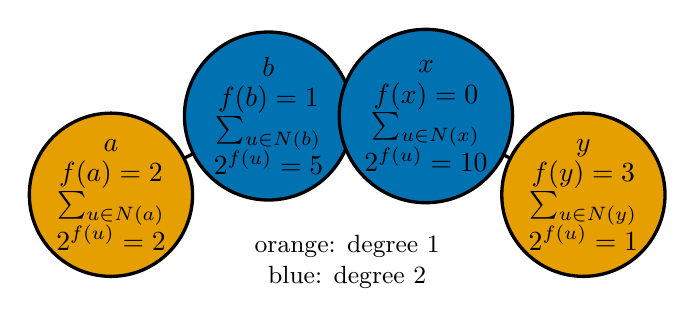
\begin{tikzpicture}[line cap=round, line join=round]
    \draw[very thick] (0,0) -- (2,1) -- (4,1) -- (6,0);
    \node[circle, draw=black, very thick, fill=oi-orange, minimum size=15mm,
      inner sep=1pt, align=center] at (0,0) {$a$\\[-1pt]$f(a)=2$\\[-1pt]
      $\sum_{u\in N(a)}$\\[-1pt]$2^{f(u)}=2$};
    \node[circle, draw=black, very thick, fill=oi-blue, minimum size=15mm,
      inner sep=1pt, align=center] at (2,1) {$b$\\[-1pt]$f(b)=1$\\[-1pt]
      $\sum_{u\in N(b)}$\\[-1pt]$2^{f(u)}=5$};
    \node[circle, draw=black, very thick, fill=oi-blue, minimum size=15mm,
      inner sep=1pt, align=center] at (4,1) {$x$\\[-1pt]$f(x)=0$\\[-1pt]
      $\sum_{u\in N(x)}$\\[-1pt]$2^{f(u)}=10$};
    \node[circle, draw=black, very thick, fill=oi-orange, minimum size=15mm,
      inner sep=1pt, align=center] at (6,0) {$y$\\[-1pt]$f(y)=3$\\[-1pt]
      $\sum_{u\in N(y)}$\\[-1pt]$2^{f(u)}=1$};
    \node[font=\small, align=center] at (3,-0.85)
      {orange: degree 1\\blue: degree 2};
  \end{tikzpicture}
  \caption{The path with vertices \(a,b,x,y\) has a labelling satisfying both required orders for \(c(i)=2^i\).}
  \label{fig:good-labelling}
\end{figure}

A degree-respecting labelling can fail the equal-degree neighbour-sum order.
In \cref{fig:bad-labelling}, the labels of the central
vertices are exchanged relative to \cref{fig:good-labelling}. The red mark
identifies a pair violating \cref{eq:equal-degree-order}, and the arrow shows
the label swap used in the proof.

\begin{figure}[ht]
  \centering
  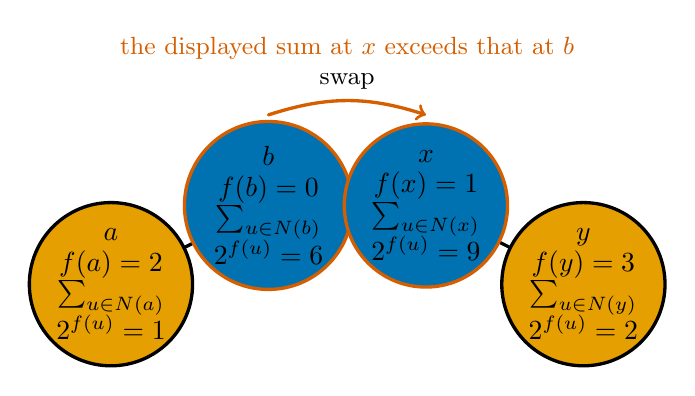
\begin{tikzpicture}[line cap=round, line join=round]
    \draw[very thick] (0,0) -- (2,1) -- (4,1) -- (6,0);
    \node[circle, draw=black, very thick, fill=oi-orange, minimum size=15mm,
      inner sep=1pt, align=center] (bad-a) at (0,0) {$a$\\[-1pt]$f(a)=2$\\[-1pt]
      $\sum_{u\in N(a)}$\\[-1pt]$2^{f(u)}=1$};
    \node[circle, draw=oi-vermillion, very thick, fill=oi-blue, minimum size=15mm,
      inner sep=1pt, align=center] (bad-b) at (2,1) {$b$\\[-1pt]$f(b)=0$\\[-1pt]
      $\sum_{u\in N(b)}$\\[-1pt]$2^{f(u)}=6$};
    \node[circle, draw=oi-vermillion, very thick, fill=oi-blue, minimum size=15mm,
      inner sep=1pt, align=center] (bad-x) at (4,1) {$x$\\[-1pt]$f(x)=1$\\[-1pt]
      $\sum_{u\in N(x)}$\\[-1pt]$2^{f(u)}=9$};
    \node[circle, draw=black, very thick, fill=oi-orange, minimum size=15mm,
      inner sep=1pt, align=center] (bad-y) at (6,0) {$y$\\[-1pt]$f(y)=3$\\[-1pt]
      $\sum_{u\in N(y)}$\\[-1pt]$2^{f(u)}=2$};
    \draw[->, very thick, oi-vermillion] (2,2.15) to[bend left=18]
      node[above, font=\small, text=black] {swap} (4,2.15);
    \node[font=\small, text=oi-vermillion, align=center] at (3,3.0)
      {the displayed sum at $x$ exceeds that at $b$};
  \end{tikzpicture}
  \caption{The same graph has a degree-respecting labelling for which \cref{eq:equal-degree-order} fails at the central pair marked by red borders; the red arrow shows the exchange of their labels.}
  \label{fig:bad-labelling}
\end{figure}

\section{Proof of Theorem~\ref{thm:strict-weights}}

Let \(\mathcal A\) be the set of all labellings that respect
\cref{eq:degree-order}. This set is nonempty. Order the vertices by
non-increasing degree, choose any order inside each degree class, and assign
the labels in \(I_n\) in that order. The set \(\mathcal A\) is finite
because it is a subset of the finite set of all bijective labellings.

For \(g\in\mathcal A\), define the edge potential
\[
  \Phi(g)=\sum_{\{x,y\}\in E}c(g(x))c(g(y)).
  \tag{4.1}\label{eq:potential}
\]
The finite nonempty set of real values \(\{\Phi(g):g\in\mathcal A\}\) has a
minimum. Choose \(f\in\mathcal A\) with minimal edge potential.

Take \(v,w\in V\) with \(d(v)=d(w)\) and \(f(w)<f(v)\). Strict increase in
\cref{eq:strict-weights} gives \(c(f(w))<c(f(v))\). Let \(f'\) be obtained from
\(f\) by exchanging the labels of \(v\) and \(w\). Since
\(d(v)=d(w)\), the exchanged labelling still belongs to \(\mathcal A\).

The edge classes used to compare \(\Phi(f')\) and \(\Phi(f)\) are shown in
\cref{fig:edge-classes}. The edge set \(E\) splits into the edges incident with
neither \(v\) nor \(w\) (\(E_0\)), with \(v\) only (\(E_v\)), with \(w\) only
(\(E_w\)), and with both (\(E_{vw}\)). Because the graph is simple,
\(E_{vw}\) is either \(\{\{v,w\}\}\) or empty.

\begin{figure}[ht]
  \centering
  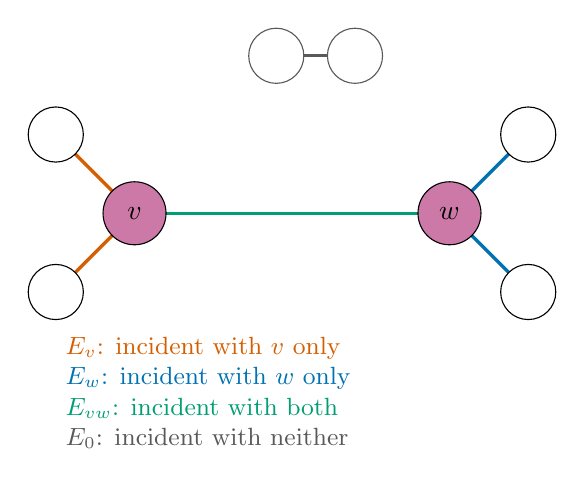
\begin{tikzpicture}[line cap=round, line join=round]
    \draw[very thick, oi-vermillion] (-1,2) -- (0,1) -- (-1,0);
    \draw[very thick, oi-blue] (4,1) -- (5,2);
    \draw[very thick, oi-blue] (4,1) -- (5,0);
    \draw[very thick, oi-green] (0,1) -- (4,1);
    \draw[very thick, black!65] (1.8,3) -- (2.8,3);
    \node[circle, draw=black, fill=oi-purple, minimum size=8mm] at (0,1) {$v$};
    \node[circle, draw=black, fill=oi-purple, minimum size=8mm] at (4,1) {$w$};
    \node[circle, draw=black, fill=white, minimum size=7mm] at (-1,2) {};
    \node[circle, draw=black, fill=white, minimum size=7mm] at (-1,0) {};
    \node[circle, draw=black, fill=white, minimum size=7mm] at (5,2) {};
    \node[circle, draw=black, fill=white, minimum size=7mm] at (5,0) {};
    \node[circle, draw=black!65, fill=white, minimum size=7mm] at (1.8,3) {};
    \node[circle, draw=black!65, fill=white, minimum size=7mm] at (2.8,3) {};
    \node[font=\small, align=left, anchor=north west] at (-1.0,-0.45)
      {\textcolor{oi-vermillion}{$E_v$: incident with $v$ only}\\
       \textcolor{oi-blue}{$E_w$: incident with $w$ only}\\
       \textcolor{oi-green}{$E_{vw}$: incident with both}\\
       \textcolor{black!65}{$E_0$: incident with neither}};
  \end{tikzpicture}
  \caption{The four colours identify the four disjoint edge classes in the edge-potential comparison for the vertices \(v\) and \(w\).}
  \label{fig:edge-classes}
\end{figure}

Edges in \(E_0\) have the same contribution before and after the exchange. The
contributions from \(E_v\) and \(E_w\), together with the unchanged contribution
from \(E_{vw}\), give
\[
  \begin{aligned}
  \Phi(f')-\Phi(f)
    &={}\bigl(c(f(w))-c(f(v))\bigr)
      \sum_{u\in N(v)\setminus\{w\}}c(f(u))\\
    &\quad+\bigl(c(f(v))-c(f(w))\bigr)
      \sum_{u\in N(w)\setminus\{v\}}c(f(u))\\
    &=\bigl(c(f(v))-c(f(w))\bigr)
      \left(
        \sum_{u\in N(w)\setminus\{v\}}c(f(u))
        -\sum_{u\in N(v)\setminus\{w\}}c(f(u))
      \right).
  \end{aligned}
  \tag{4.4}\label{eq:swap-identity}
\]
Minimality of \(f\) gives \(\Phi(f')-\Phi(f)\geq0\). Since
\(c(f(v))-c(f(w))>0\), \cref{eq:swap-identity} implies
\[
  \sum_{u\in N(v)\setminus\{w\}}c(f(u))
  \leq
  \sum_{u\in N(w)\setminus\{v\}}c(f(u)).
  \tag{4.5}\label{eq:neighbour-sums-except}
\]

We distinguish whether \(v\) and \(w\) are adjacent.

\paragraph{Adjacent case.}
If \(v\sim w\), then
\[
  \begin{aligned}
  \sum_{u\in N(v)}c(f(u))
    &=\sum_{u\in N(v)\setminus\{w\}}c(f(u))+c(f(w))\\
    &\leq\sum_{u\in N(w)\setminus\{v\}}c(f(u))+c(f(v))\\
    &=\sum_{u\in N(w)}c(f(u)).
  \end{aligned}
\]
Thus the required inequality holds in the adjacent case.

\paragraph{Non-adjacent case.}
If \(v\not\sim w\), then
\[
  \sum_{u\in N(v)}c(f(u))
  =\sum_{u\in N(v)\setminus\{w\}}c(f(u))
  \leq\sum_{u\in N(w)\setminus\{v\}}c(f(u))
  =\sum_{u\in N(w)}c(f(u)).
\]
Thus the required inequality holds in the non-adjacent case. Therefore \(f\) satisfies
\cref{eq:equal-degree-order}, which proves \cref{thm:strict-weights}.

\section{Proof of Corollary~\ref{cor:powers-of-two}}

Apply \cref{thm:strict-weights} to the function
\[
  c(i)=2^i\qquad(i\in I_n).
  \tag{5.1}\label{eq:powers-function}
\]
This function is strictly increasing. The resulting inequalities are exactly
the degree condition and the displayed inequality in the corollary.

\section{Scope and limitations}

The argument includes the empty graph and graphs with vertices but no edges.
The conclusions assert existence and do not assert uniqueness. The minimiser
of the edge potential defined in \cref{eq:potential} is one
construction among possibly many labellings satisfying the degree order and the
equal-degree neighbour-sum order. In the swap argument, \(f(w)<f(v)\) gives
\(c(f(w))<c(f(v))\). This is the step requiring strict weights. A non-decreasing
function need not satisfy this strict inequality, so non-decreasing weights are outside the
scope of the stated theorem.

\section{Formal verification}

A companion machine-checked proof written in the Lean 4 proof assistant
formalises the definitions and proves the two theorems. It also formalises the
finite-minimisation and label-swap lemmas. The formal representation treats the
finite vertex set as a finite type, which is a set
equipped with a finite enumeration, and uses an ordered set of \(n\) positions
for labels. The weights are represented by a strictly increasing real-valued
function on that ordered label set. The formal development relies on three
foundational principles: propositional extensionality, which identifies
logically equivalent propositions; choice, which selects an element from a
nonempty collection; and quotient soundness, which supplies equality for
equivalent representatives. These are proof dependencies, not hypotheses on
the graph or on the weights. The Lean names of these principles are
\texttt{propext}, \texttt{Classical.choice}, and \texttt{Quot.sound}.

Each vertex is represented by one position in the finite
ordered type, and a labelling is a bijection to that type. The edge potential is
represented by a finite sum over the edge set.
The Lean development formalises the minimisation argument and label-swap
calculation.

\bibliographystyle{amsplain}
\bibliography{../references}

\end{CJK*}
\end{document}
